\documentclass[usenames,dvipsnames]{beamer}

\usepackage{acronym}
\usepackage[backend=bibtex]{biblatex}
\usepackage{default}
\usepackage{graphicx}
\usepackage[utf8]{inputenc}
\usepackage{listings}
\usepackage{lmodern}
\usepackage{nameref}
\usepackage{textcomp}

\graphicspath{{figures/}}
\acrodef{CAS}{Compare-And-Swap}
\acrodef{DCAS}{Double-Compare-And-Swap}
\acrodef{DCSS}{Double-Compare-Single-Swap}
\acrodef{DS}{Data Structure}
\acrodef{FAA}{Fetch-And-Add}
\acrodef{FAO}{Fetch-And-Or}
\acrodef{PQ}{Priority Queue}
\acrodef{TAS}{Test-And-Set}

\bibliography{../common/bibliography.bib}

\setbeamertemplate{bibliography item}{}

\lstset{
    language=C++,
    basicstyle=\ttfamily,
    keywordstyle=\color{OliveGreen},
    commentstyle=\color{Gray},
    captionpos=b,
    breaklines=true,
    breakatwhitespace=false,
    showspaces=false,
    showtabs=false,
    numbers=none,
}

\title{Concurrent Priority Queues}
\subtitle{Seminar in Algorithms, 2013W}
\author{Jakob Gruber, 0203440}
\date{\today}

\begin{document}

\maketitle

\begin{frame}{Outline}
\begin{minipage}[t][10em][t]{\linewidth}
\tableofcontents
\end{minipage}
\end{frame}

% --------------------------------------------------------------------------------------------------
\section{Introduction} \label{sec:intro}
% --------------------------------------------------------------------------------------------------

\begin{frame}[fragile,allowframebreaks]{\nameref{sec:intro}}
\acp{PQ}:

\begin{itemize}
\item Standard abstract data structure
\item Used widely in algorithmics, operating systems, task scheduling, etc
\item Interface consists of two $O(\log n)$ operations:

\begin{lstlisting}
void Insert(pq_t *pq, key_t k, value_t v)
bool DeleteMin(pq_t *pq, value_t *v)
\end{lstlisting}

\item Typical backing data structures: heaps \& search trees
\end{itemize}

\framebreak

\begin{itemize}
\item In the past decade, processor clock speeds have remained the same, trend towards multiple cores
\item New data structures required to take advantage of concurrent execution
\item The topic of this presentation: efficient concurrent \acp{PQ}
\item Fine-grained locking \textrightarrow ~ Lock-free \textrightarrow ~ Relaxed data structures
\end{itemize}

\end{frame}

\begin{frame}{Concepts and Definitions}
\framesubtitle{Safety conditions: nothing bad has happened yet}

\begin{itemize}
\item \emph{Linearizability}: operations appear to take effect at a single point in time, the linearization point
\item \emph{Quiescent consistency}: in a period of quiescence, semantics equivalent to some sequential ordering
\item And others, i.e. \emph{sequential consistency}, \emph{serializability}
\end{itemize}
\end{frame}

\begin{frame}{Concepts and Definitions}
\framesubtitle{Liveness conditions: something good eventually happens}

\begin{itemize}
\item \emph{Lock-freedom}: at least a single process makes progress at all times
\item \emph{Wait-freedom}: every process finishes in a bounded number of steps
\item Further liveness conditions: \emph{Starvation-freedom}, \emph{Deadlock-freedom}
\end{itemize}
\end{frame}

\begin{frame}{Concepts and Definitions}
\framesubtitle{Miscellaneous}

\begin{itemize}
\item \emph{Disjoint-access parallelism}: how well a data structure handles concurrent use by multiple
      threads within disjoint areas
\item Synchronization primitives:
    \begin{itemize}
    \item \ac{CAS}, \ac{FAA}, \ac{FAO}, \ac{TAS}
    \item \ac{DCAS}, \ac{DCSS}
    \end{itemize}
\end{itemize}
\end{frame}

% --------------------------------------------------------------------------------------------------
\section{Related Work} \label{sec:related}
% --------------------------------------------------------------------------------------------------

\begin{frame}{\nameref{sec:related}}
\begin{itemize}
\item Non-standard synchronization primitives
    \begin{itemize}
    \item \citeauthor{liu2012lock}: Array-based \ac{PQ} with \lstinline|ExtractMany|
    \item \citeauthor{israeli1993efficient}: Wait-free \ac{PQ}
    \end{itemize}

\item Bounded range priorities
    \begin{itemize}
    \item \citeauthor{shavit1999scalable}: Combining funnels \& bins
    \end{itemize}

\item \acp{PQ} in distributed memory systems
    \begin{itemize}
    \item \citeauthor{sanders1998randomized}: Local \acp{PQ}, \lstinline|Insert| at random processor
    \end{itemize}

\item Relaxed data structures
    \begin{itemize}
    \item \citeauthor{kirsch2012fast}: k-FIFO queues
    \end{itemize}

\end{itemize}
\end{frame}

% --------------------------------------------------------------------------------------------------
\section{Fine-grained Locking Heaps} \label{sec:locking}
% --------------------------------------------------------------------------------------------------

\begin{frame}{\nameref{sec:locking}}
\framesubtitle{\citeauthor{hunt1996efficient}}

\begin{itemize}
\item Naive \ac{PQ} parallelization: single global lock \textrightarrow ~ sequential bottleneck
\item A first improvement: fine-grained locking using a lock per node
\item \fullcite{hunt1996efficient}
\end{itemize}
\end{frame}

\begin{frame}{\nameref{sec:locking}}
\framesubtitle{\citeauthor{hunt1996efficient}: Innovations}

\begin{itemize}
\item One lock per node, \emph{but} additionally a global lock protecting the heap's
      \lstinline|size| variable
\item Insertions bottom-up, deletions top-down to reduce contention
\item Successive insertions take disjoint paths towards the root
\end{itemize}
\end{frame}

\begin{frame}{\nameref{sec:locking}}
\framesubtitle{\citeauthor{hunt1996efficient}: Limitations}

\begin{itemize}
\item A global lock remains
\item Heap is statically allocated
\item Frequent complex heap reorganization
\item Disjoint-access breaks down at high traffic levels
\item Inherent \ac{PQ} bottleneck at the minimal node
\item Benchmarks show only limited scalability up to a low thread count
\end{itemize}
\end{frame}

% --------------------------------------------------------------------------------------------------
\section{Lock-free Priority Queues} \label{sec:lockfree}
% --------------------------------------------------------------------------------------------------

\begin{frame}{\nameref{sec:lockfree}}
\framesubtitle{SkipLists}

\begin{itemize}
\item Modern concurrent \acp{PQ} are mostly based on \citeauthor{pugh1990skip}'s \ac{SL}
\item Probabilistic ordered search structure, insertions and deletions in expected $O(\log n)$ time
\item No reorganizations
\item Simple implementation
\item Excellent disjoint-access properties
\end{itemize}
\end{frame}

\begin{frame}[fragile]{\nameref{sec:lockfree}}
\framesubtitle{SkipLists}

\begin{itemize}
\item Collection of linked lists with corresponding levels
\item Lowest list contains all items, higher lists are shortcuts
\item \lstinline|Insert| chooses a \lstinline|level| according to geometric distribution
\end{itemize}

\begin{lstlisting}
struct slist_t {
  size_t max_level;
  node_t head[max_level];
};
struct node_t {
  key_t key;
  value_t value;
  size_t level;
  node_t *next[level];
};
\end{lstlisting}
\end{frame}


\begin{frame}{\nameref{sec:lockfree}}
\framesubtitle{\citeauthor{shavit2000skiplist}}

\begin{itemize}
\item First SkipList-based \ac{PQ}
\item \fullcite{shavit2000skiplist}
\item Initially lock-based, lock-free variant published in 2008
\item \fullcite{herlihy2012art}
\end{itemize}
\end{frame}

\begin{frame}{\nameref{sec:lockfree}}
\framesubtitle{\citeauthor{shavit2000skiplist}}

\begin{figure}
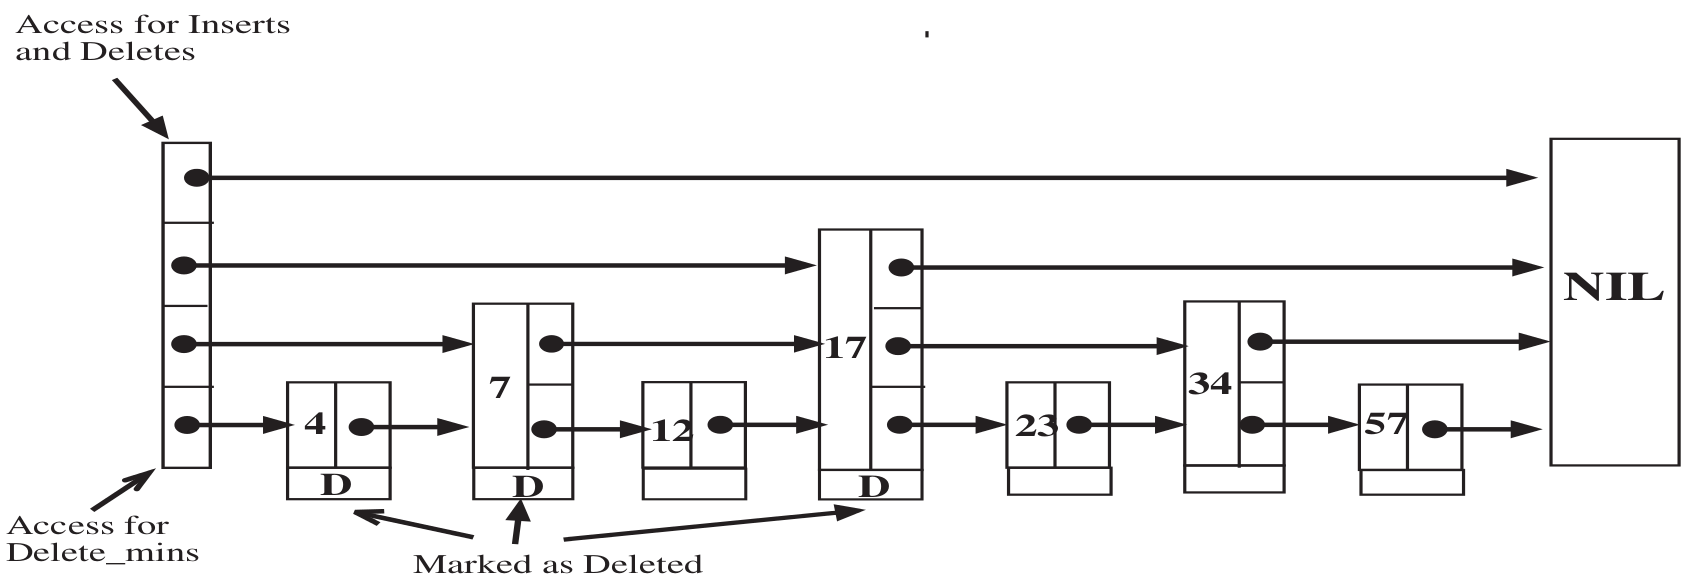
\includegraphics[width=\textwidth]{shavit_lotan}
\caption{The \citeauthor{shavit2000skiplist} \ac{PQ} (Image source: \cite{shavit2000skiplist})}
\end{figure}
\end{frame}

\begin{frame}{\nameref{sec:lockfree}}
\framesubtitle{\citeauthor{shavit2000skiplist}}

\begin{itemize}
\item Items are considered in the list once inserted on bottom level
\item Again, insertions bottom-up and deletions top-down
\item Deletions are split
    \begin{itemize}
    \item Logical deletion sets a \lstinline|deleted| flag
    \item Physical deletion performs actual pointer manipulations
    \end{itemize}
\item \lstinline|DeleteMin| attempts to logically delete the head node.
     On success: delete physically \& return node. Otherwise, continue with
     next node.
\item \lstinline|Insert| is equivalent to the \ac{SL} insertion
\end{itemize}
\end{frame}

\begin{frame}{\nameref{sec:lockfree}}
\framesubtitle{\citeauthor{shavit2000skiplist}}

\begin{itemize}
\item
\end{itemize}
\end{frame}

\begin{frame}{\nameref{sec:lockfree}}
\framesubtitle{\citeauthor{shavit2000skiplist}}

\begin{itemize}
\item
\end{itemize}
\end{frame}

% --------------------------------------------------------------------------------------------------
\section{Relaxed Priority Queues} \label{sec:relaxed}
% --------------------------------------------------------------------------------------------------

\begin{frame}{\nameref{sec:relaxed}}

\end{frame}

% --------------------------------------------------------------------------------------------------
\section{Conclusion} \label{sec:conclusion}
% --------------------------------------------------------------------------------------------------

\begin{frame}{\nameref{sec:conclusion}}

\end{frame}

% --------------------------------------------------------------------------------------------------
\section{References} \label{sec:references}
% --------------------------------------------------------------------------------------------------

\begin{frame}[allowframebreaks]{\nameref{sec:references}}
\printbibliography
\end{frame}

\end{document}
